\documentclass[../sk-egzamin.tex]{subfiles}

\begin{document}

\question{
Proszę opisać, jak działa podpis cyfrowy.
}

% TODO: replace with tikz
\begin{center}
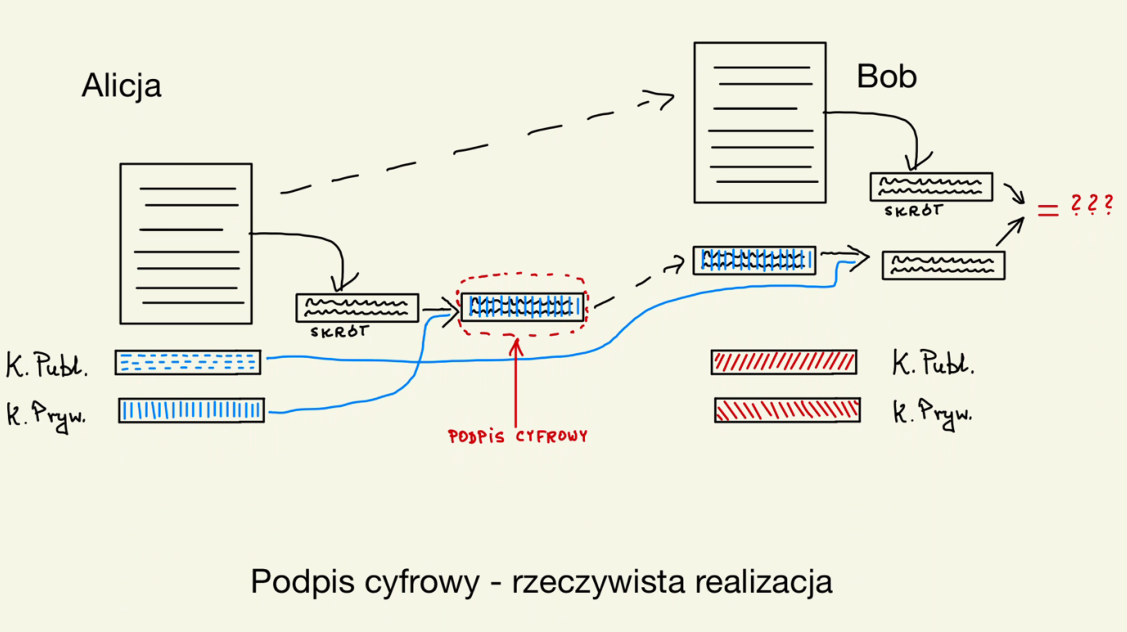
\includegraphics[width=\textwidth]{podpis}
\end{center}

\begin{itemize}
    \item Zaszyfrowanie \textbf{kluczem prywatnym} daje gwarancję,
    że zaszyfrowana wiadomość \textbf{pochodzi z odpowiedniago źródła}.

    % \item Samej podpisywanej wiadomości nie musi się szyfrować.

    \item Generowany jest jej skrót i ten \textbf{skrót jest szyfrowany}
    z wykorzystaniem klucza \textbf{prywatnego} osoby podpisującej.

    \item \textbf{Zaszyfrowany skrót stanowi podpis cyfrowy.}

    \item Niezaszyfrowana wiadomość może być przesłana jawnie razem z
    zaszyfrowanym skrótem (czyli podpisem cyfrowym).

    \item Odbiorca wykonuje dwie czynności:
    \begin{enumerate}
        \item Odszyfrowuje skrót używając klucza \textbf{publicznego nadawcy}
        (klucz ten jest powszechnie znany, a w każdym razie dostępny).

        \item \textbf{Tworzy skrót} wiadomości używając tej samej funkcji
        haszującej.
    \end{enumerate}

    \item Jeśli wyniki obu operacji są identyczne, to znaczy, że wiadomość
    na pewno podpisał określony nadawca, a ponadto nikt po tej wiadomości nie
    zmienił już po podpisaniu.
\end{itemize}

% Po podpisaniu dodatkowo możemy wiadomość zaszyfrować, ale to nie
% należy już do samego podpisu.
% Jeśli wiadomość jest duża, to najlepiej szyfrować go okresowo zmienianym kluczem
% symetrycznym, przy czym samo uzgodnienie kluczy jest realizowane przy pomocy
% szyfrowania z kluczem publicznym i prywatnym.


\pagebreak
\end{document}
